\subsection{Trang chủ}
Đầu tiên là giao diện \textbf{Trang chủ}, là nơi trò chơi hiển thị đầu tiên khi người chơi khởi động:
\begin{figure}[H]
    \centering
    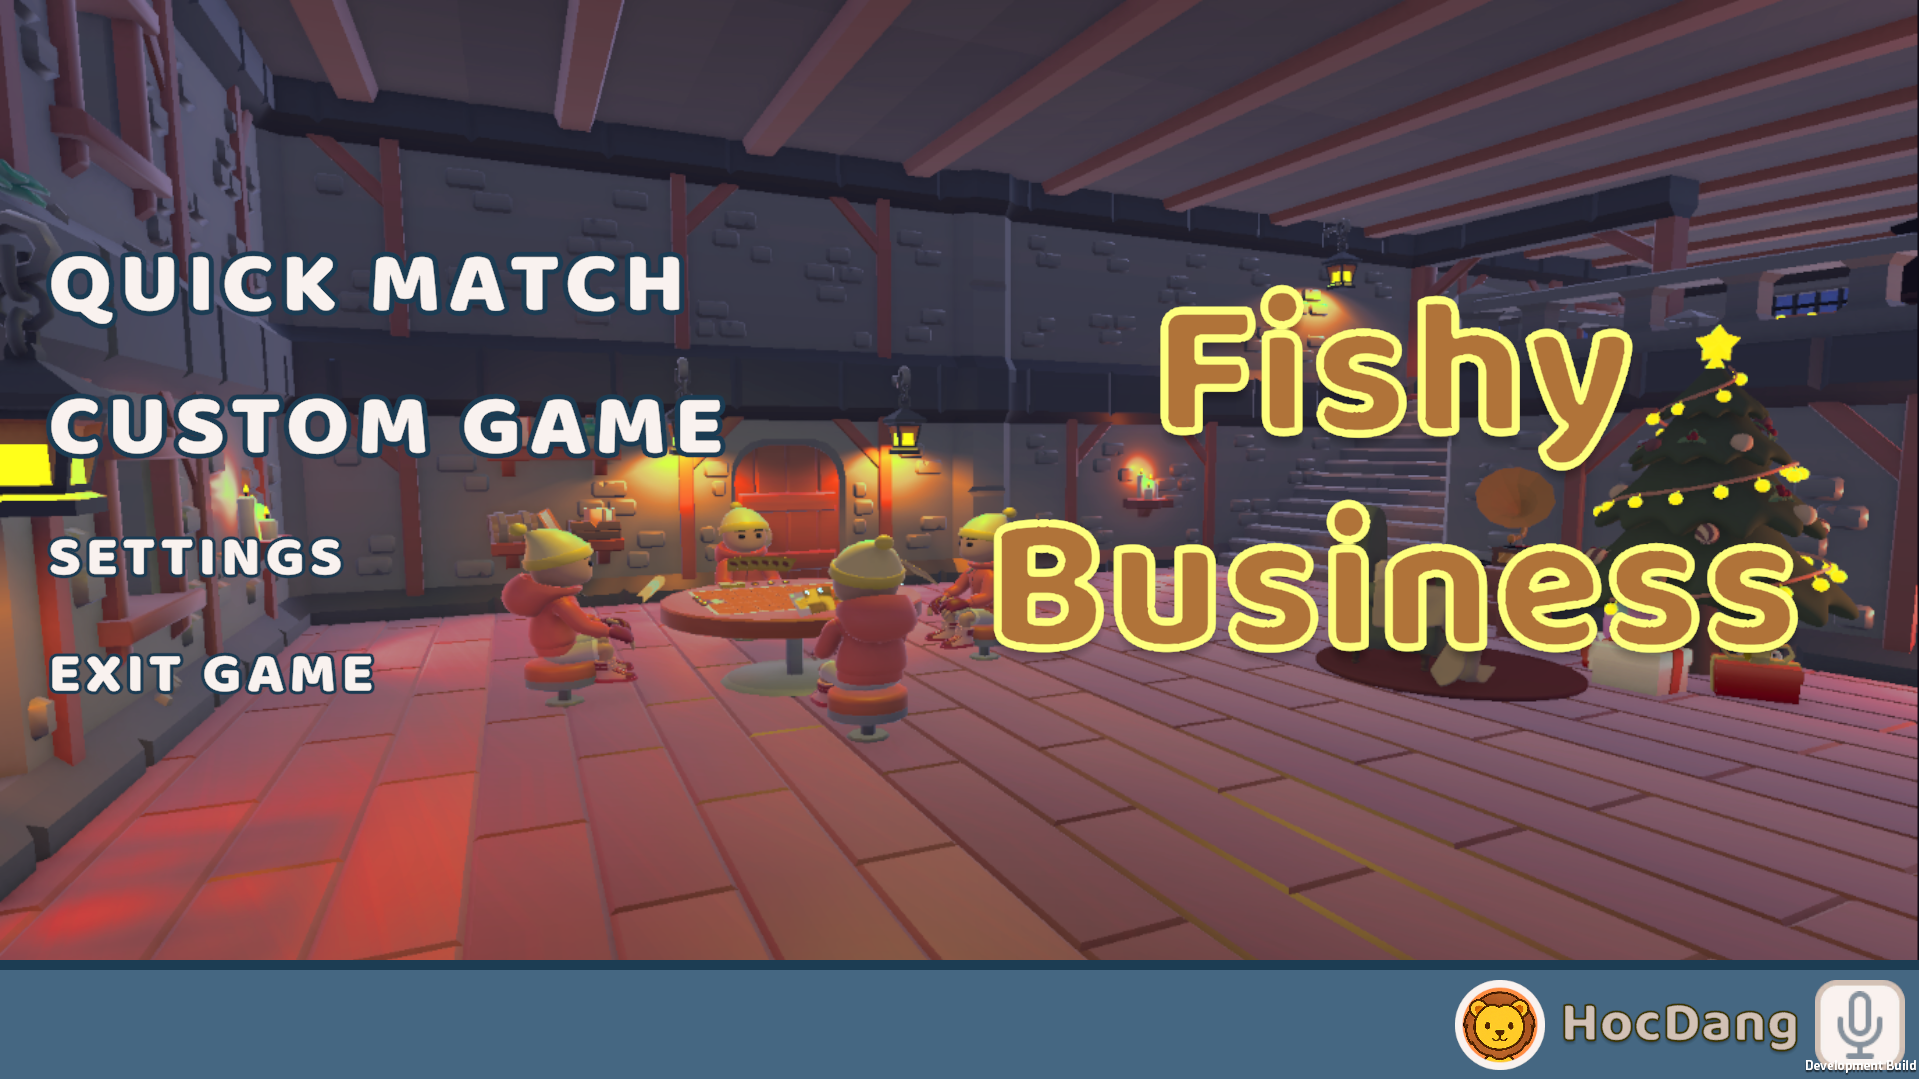
\includegraphics[width=0.75\linewidth]{10.Kết quả/images/MainMenu.png}
    \caption{Screenshot màn hình \textbf{Trang chủ} của trò chơi}
    \label{fig:game-object}
\end{figure}
Tại đây, người chơi có thể chọn:
\begin{itemize}
    \item \textbf{Quick Match} để tham gia vào 1 phòng chơi ngẫu nhiên (nếu có), 
    \item \textbf{Custom Game} để xem các phòng chơi hiện có và tham gia 1 phòng chơi trong số đó hoặc tạo 1 phòng chơi mới,
    \item  \textbf{Settings} để điều chỉnh các thống số hệ thống. 
    \item \textbf{Exit Game} để thoát trò chơi.
\end{itemize}

Ở góc dưới bên phải màn hình sẽ là thông tin của người chơi, người chơi có thể thay đổi thông tin bằng cách nhấn vào góc dưới đó.

\begin{figure} [H]
    \centering
    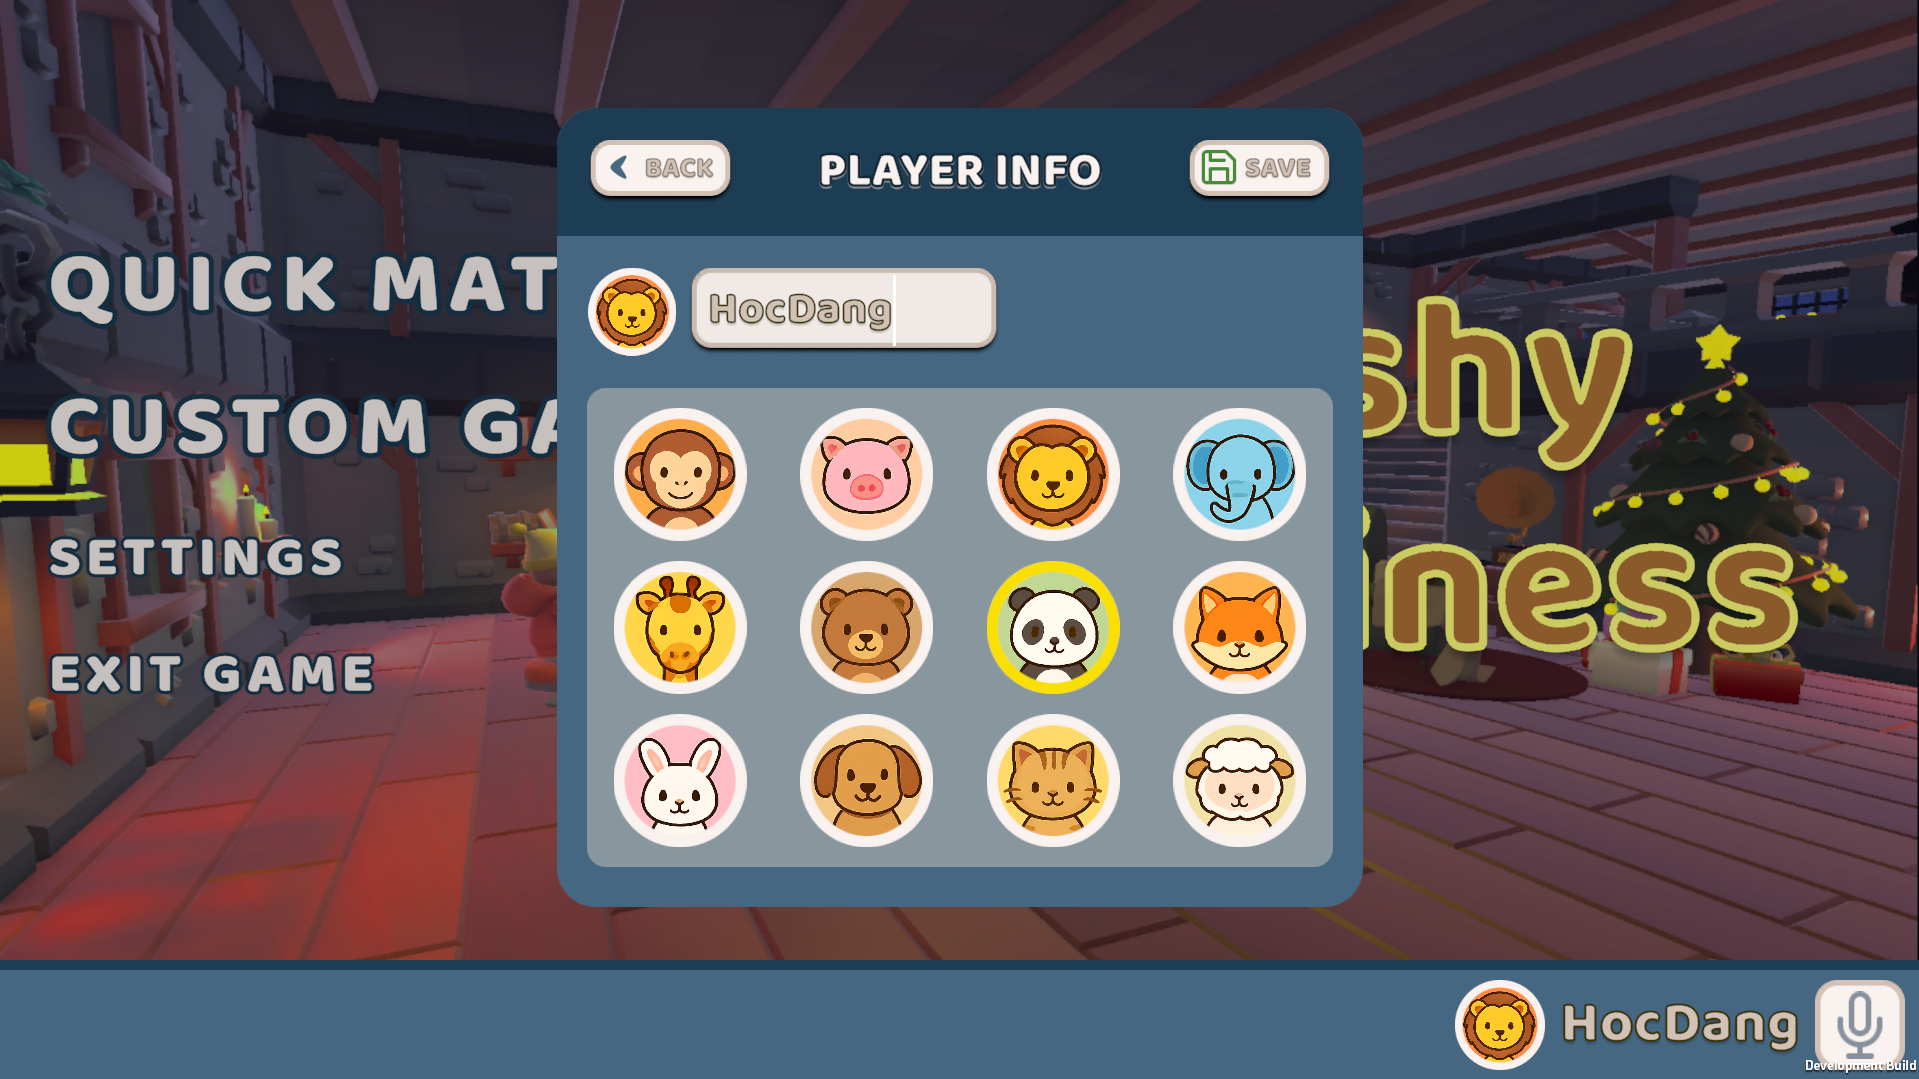
\includegraphics[width=0.75\linewidth]{10.Kết quả//images/ChangeName&Icon.png}
    \caption{Screenshot màn hình thay đổi tên và icon}
    \label{fig:placeholder}
\end{figure}

Sau khi nhấn nút \textbf{Custom Game} từ trang chủ, hệ thống hiển thị danh sách các phòng chơi hiện có như hình dưới đây:
\begin{figure}[H]
    \centering
    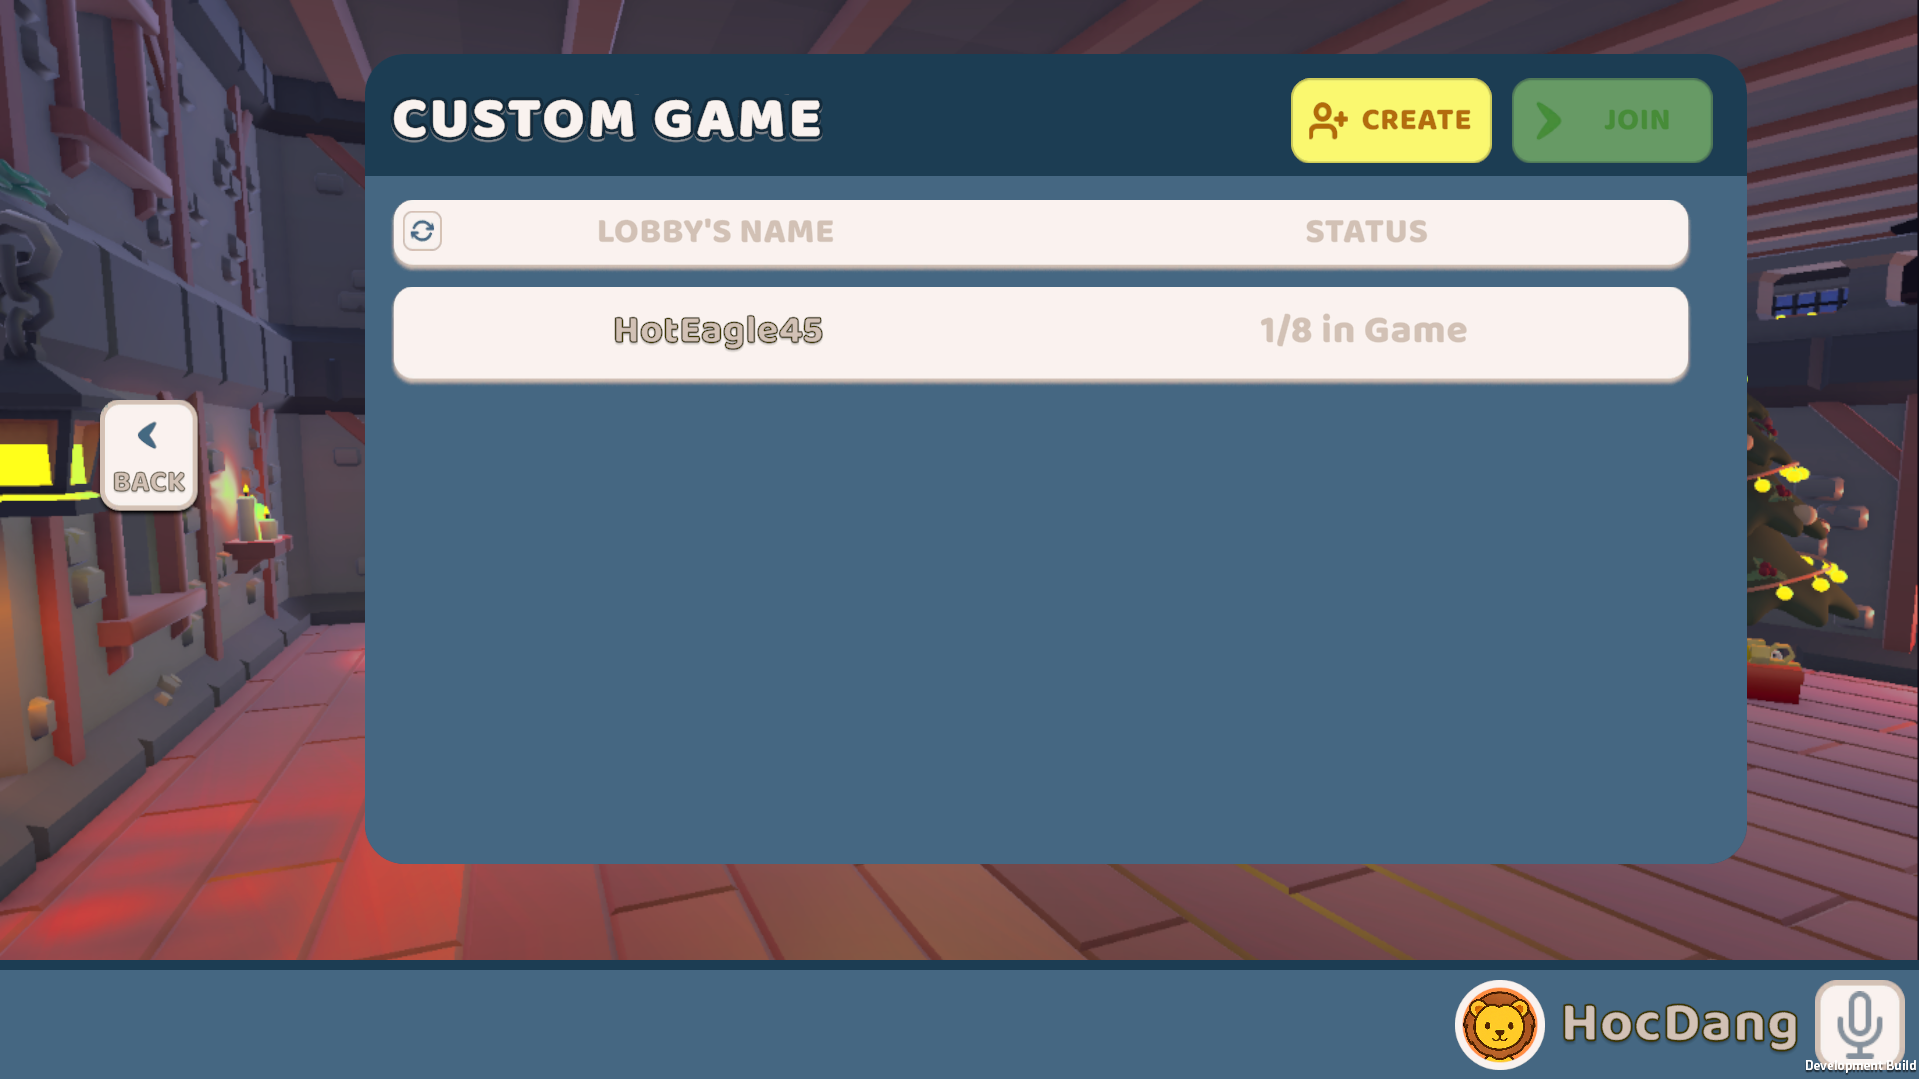
\includegraphics[width=0.75\linewidth]{10.Kết quả/images/CustomGame.png}
    \caption{Screenshot màn hình \textbf{Custom Game} của trò chơi}
    \label{fig:game-object}
\end{figure}
Ở giao diện này, người chơi có thể chọn 1 phòng chơi hiện có và chưa đầy người chơi (8 người) và nhấn nút \textbf{Join} để tham gia vào phòng chơi đó. Người chơi cũng có thể chọn \textbf{Create} để tạo phong chơi mới.
\begin{figure}[H]
    \centering
    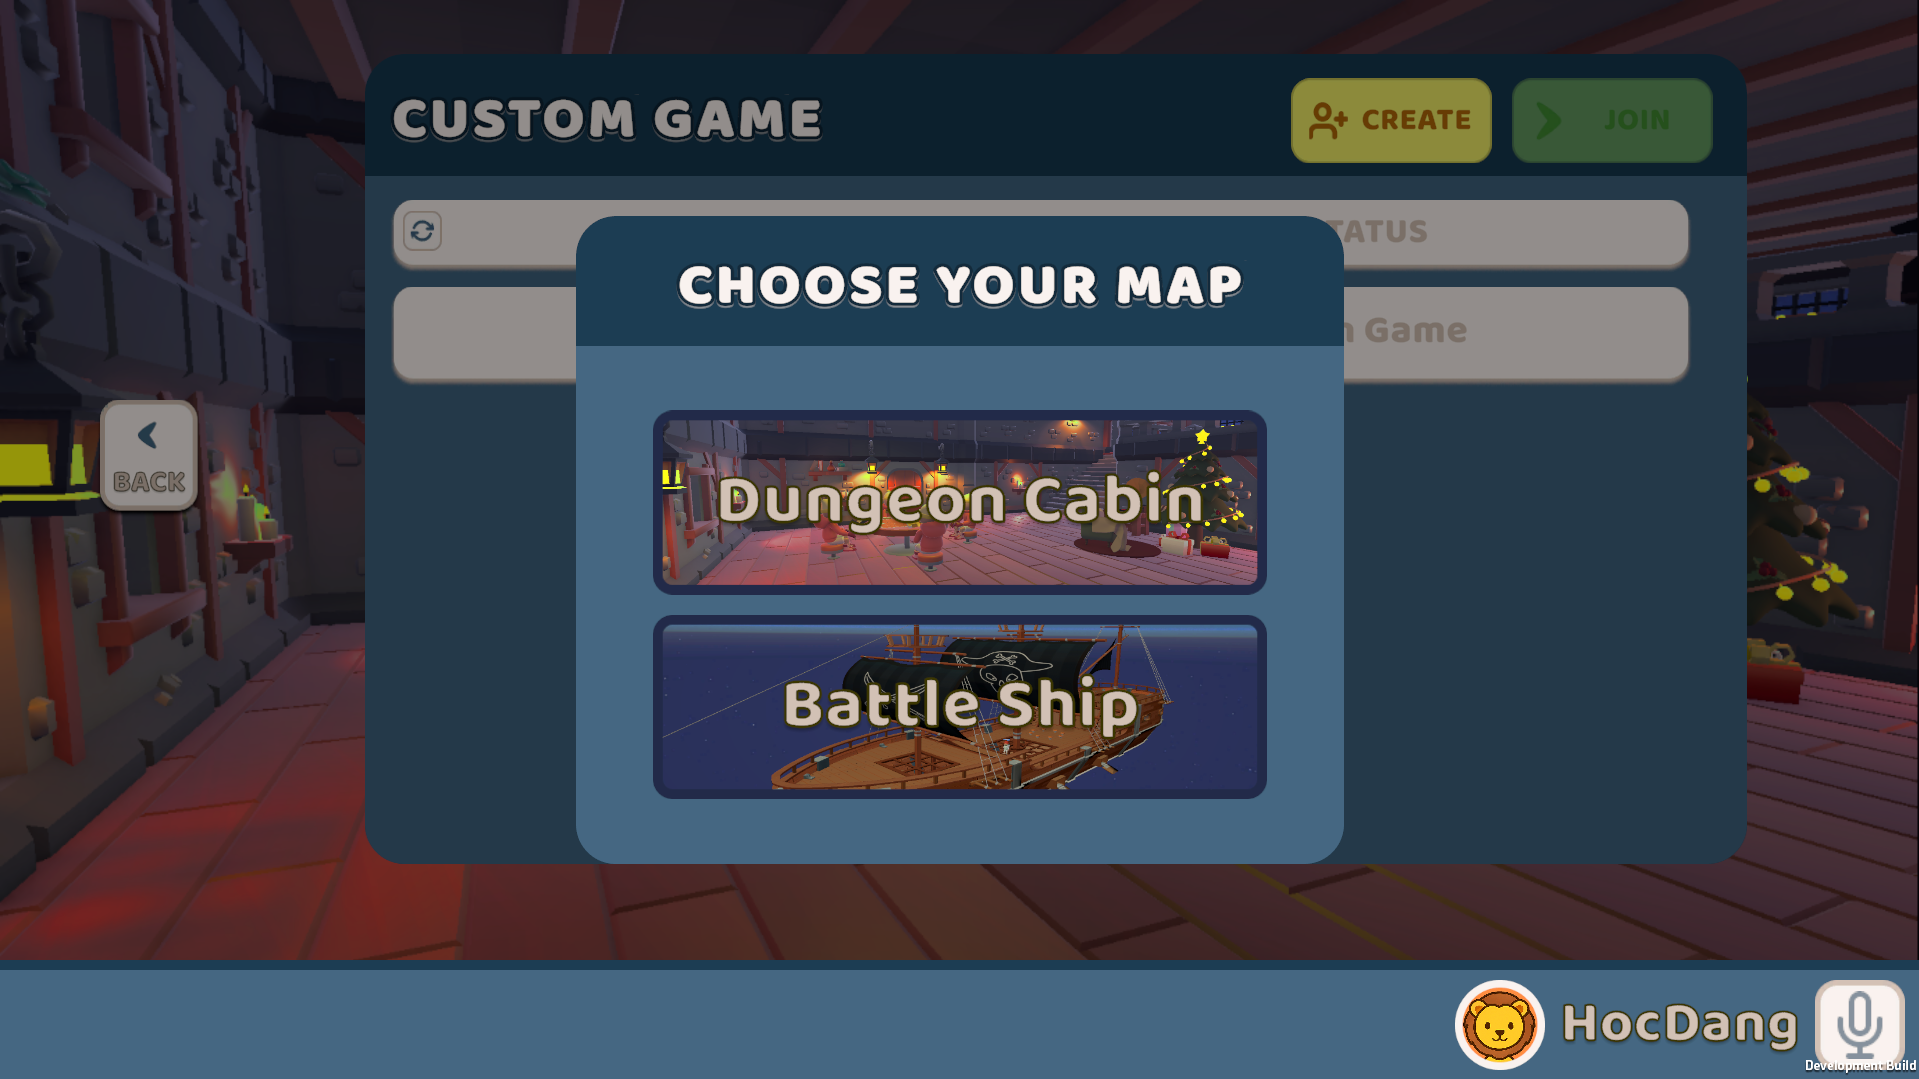
\includegraphics[width=0.75\linewidth]{10.Kết quả/images/ChooseMap.png}
    \caption{Screenshot màn hình chọn bản đồ của trò chơi}
    \label{fig:game-object}
\end{figure}
Tại đây, người chơi có thể chọn 1 trong 2 bản đồ để hoàn thành tạo 1 phòng chơi với bản đồ đó.